\section{INTRODUÇÃO}
\subsection{Contextualização}

A Teoria Geral dos Sistemas (T.G.S) ou General Theory of Systems foi proposta pelo Biólogo Autríaco Karl Ludwig Von Bertalanffy em 1940, desenvolveu seu trabalho até meados de 1948, quando se mudou para América do Norte. Em 1956 Ross Ashby introduziu o conceito na ciência cibernética. A pesquisa de Von Bertalanffy foi baseada numa visão diferente do reducionismo científico até então aplicada pela ciência convencional. Dizem alguns que foi uma reação contra o reducionismo e uma tentativa para criar a unificação científica (BERTALANFFY, 2008) e (COSTA,2020).\vskip0.3cm

A ideia de sistema tem uma longa trajetória, remonta a Antiguidade, com pensadores como Aristóteles “o todo é maior que a soma de suas partes”, Platão e Sócrates, que já se utilizavam desse conceito à medida que procuravam formas de compreender e explicar os acontecimentos, fenômenos da natureza e o comportamento humano.\vskip0.3cm

O princípio geral da teoria é que um sistema não pode ser compreendido apenas pela análise de suas partes isoladamente, pois o comportamento do todo depende das interações e das relações entre essas partes. Essa perspectiva influenciou diversas áreas, como biologia, sociologia, psicologia, administração e ciência da computação.\vskip0.3cm



As aplicações da Teoria Geral dos Sistemas teve início nos Estados Unidos da América (USA) com aplicações à: - Biologia - Termodinâmica.\vskip0.3cm

Alguns anos a frente sua aplicação se fez presente em outras áreas, tais como:

\begin{itemize}
    \item Ecologia (TANLEY, 1937);
    \item Geografia (SOTCHAVA, 1977);
    \item Psicologia Social das Organizações (KATZ e KAHN, 1966);
    \item Psiquiatria (GRINKER, 1967);
    \item Psicologia do Desenvolvimento (BRONFRENBRENNER, 1977);
    \item Economia (BOULDING, 1953);
    \item Administração (SCOTT, 1963);
\end{itemize}

\newpage
\subsection{Panorama do Marketing Digital Global}


A mídia social e o conteúdo gerado pelo usuário definem tecnologias interativas projetadas para criar e compartilhar informações, ideias e interesses entre comunidades virtuais. A mídia social varia de acordo com postagens de texto, imagens, vídeos, comentários e plataformas de rede. A taxa de penetração global atingiu 66,2\% e 5,22 bilhões de usuários de mídia social em todo o mundo em 2024. O norte e o oeste da Europa tiveram a maior taxa de penetração, seguidos pelo leste da Ásia e pelo sul da Europa. A Ásia ostenta hoje, quase três bilhões de usuários de mídia social, tornando-se o continente com maior audiência (STATISTICA, 2024).\vskip0.3cm

Segundo o Relatório de Visão Geral Global Digital da DataReportal(2024), em dezembro de 2024, as redes sociais mais populares, por números de usuários ativos mensais (em milhões) eram:


\begin{enumerate}
    \item Facebook = 3.065
    \item YouTube = 2,504
    \item WhatsApp = 2,000
    \item TikTok = 1,582
    \item WeChat = 1,343
    \item Facebook Messenger = 1,010
    \item Telegram = 900
\end{enumerate}

No Brasil, 62,3\% da população utiliza pelo menos uma rede social, indicando que ainda há espaço para crescimento. Já em relação aos aplicativos, há uma dominância do WhatsApp, utilizado por 83,2\% dos usuários no mundo (DATAREPORTAL, 2024). \vskip0.3cm

\begin{enumerate}
    \item WhatsApp = 83,2\%
    \item Facebook = 64,1\%   
    \item YouTube = 63,7\%
    \item Line = 62,9\%
    \item TikTok = 61,7\%
\end{enumerate}

\newpage

Em relação ao tempo médio mensal gasto por usuário usando redes sociais, verificou-se que, o TikTok estar no topo do ranking, cerca de 34 horas, o que representa mais de uma hora por dia. Na sequência, aparecem o YouTube (28 horas e 5 minutos) e Facebook (19 horas e 47 minutos).  \vskip0.3cm


Esses números refletem a popularidade e o alcance global dessas plataformas em 2024.





\subsection{Apresentação do TikTok como Objeto de Estudo}

O TikTok, lançado inicialmente como Douyin na China em setembro de 2016 pela empresa ByteDance, rapidamente se transformou em uma das plataformas de mídia social mais influentes e populares do mundo. A versão internacional do app, com o nome de TikTok, foi apresentada ao público global em setembro de 2017. A plataforma foi projetada para permitir que os usuários criassem e compartilhassem vídeos curtos, com duração de até 60 segundos, normalmente acompanhados de músicas, efeitos especiais e desafios virais 
 (KAYE et al, 2020).\vskip0.3cm

A ascensão meteórica do TikTok foi acelerada em 2018, quando a ByteDance adquiriu o aplicativo musical.ly, que já era bastante popular entre adolescentes no Ocidente. A fusão das duas plataformas resultou na criação de um ambiente único, onde usuários de diferentes partes do mundo podiam se conectar e interagir por meio de vídeos criativos e espontâneos.\vskip0.3cm

A proposta inovadora do TikTok, que combina algoritmos poderosos de recomendação com uma interface simples e intuitiva, foi um dos principais fatores de seu sucesso. A plataforma é alimentada por um algoritmo de inteligência artificial que personaliza a experiência de cada usuário, exibindo conteúdos que têm mais chances de gerar engajamento, o que aumenta a quantidade de tempo que as pessoas passam no aplicativo.\vskip0.3cm

Em poucos anos, o TikTok se transformou em uma verdadeira potência da mídia social, com mais de 1,582 bilhão de usuários ativos mensais, influenciando não apenas o comportamento dos usuários, mas também a indústria musical, a publicidade e até mesmo a cultura pop global. Ele se tornou um espaço para lançamentos de tendências, campanhas de marketing inovadoras e expressão pessoal criativa, consolidando-se como um fenômeno global, especialmente entre a geração Z (STATISTICA, 2024).\vskip0.3cm

\newpage
\subsection{Restrições de Uso em Países}

O TikTok, uma das redes sociais mais populares do mundo, tem enfrentado diversas restrições e bloqueios em vários países devido a questões de segurança nacional, privacidade de dados e preocupações com o conteúdo gerado pelos usuários, até questões culturais e religiosas.\vskip0.3cm

Elas podem ser classificadas em três categorias principais: bloqueios totais, restrições parciais e limitações específicas para determinados usuários ou grupos.


\subsubsection{India}

Em 2020, o TikTok foi banido indefinidamente na Índia após o país ter um confronto de fronteira com a China. O banimento ocorreu após um aumento das tensões entre Índia e China devido a um confronto militar na região de Ladakh. As autoridades indianas alegaram preocupações de segurança cibernética e proteção de dados, argumentando que esses aplicativos poderiam representar um risco para a soberania e integridade do país.
\vskip0.3cm

\begin{figure}[H]
    \centering
    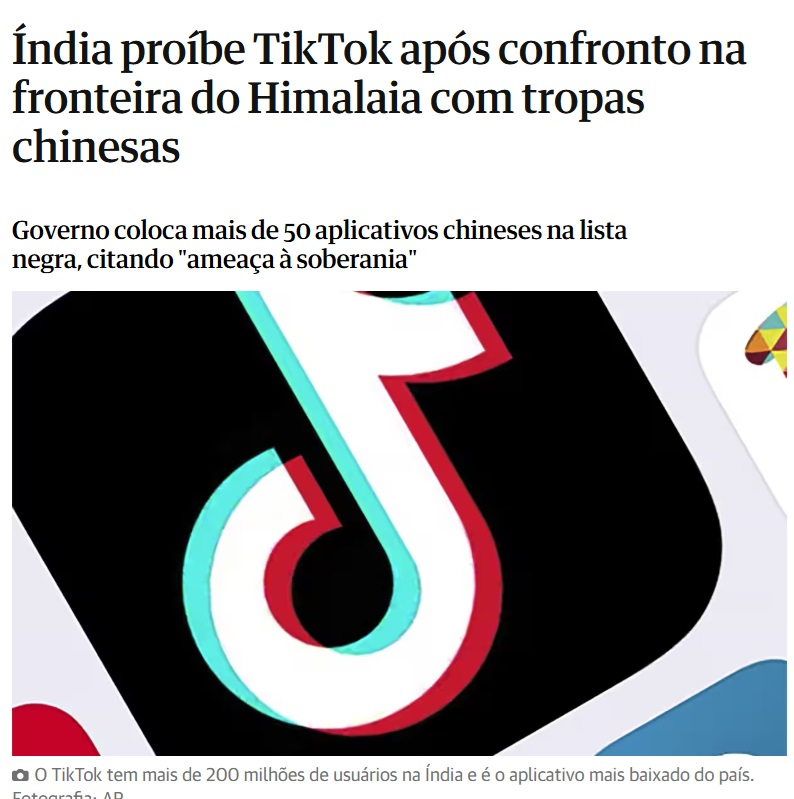
\includegraphics[width=0.7\linewidth]{TIKTOK1.jpg}
    \caption{Bloqueio do TikTok na India (The Gardian, 2020)}
    \label{fig:enter-label} 
\end{figure}


\subsubsection{Afeganistão}

A liderança Talibã do Afeganistão proibiu o TikTok e o jogo PUBG em 2022, com o argumento de proteger os jovens de "serem enganados". Essa ação reflete o controle rígido que o Talibã busca impor sobre a sociedade e as ferramentas digitais desde que voltou ao poder em agosto de 2021.


\subsubsection{Taiwan}

Em dezembro de 2022, Taiwan impôs uma proibição do setor público ao TikTok depois que o FBI alertou que o TikTok representava um risco à segurança nacional.


\subsubsection{Canadá}
Em 6 de novembro de 2024, o Canadá ordenou que o TikTok encerrasse seus escritórios no país devido a preocupações de segurança nacional, mas o acesso ao aplicativo não foi proibido. No entanto, os usuários ainda poderão acessar o aplicativo de vídeo e carregar conteúdo nele.







